% Random Geometry Problem
\begin{center}
    \textbf{\Huge Random Geometry Problem}\\
    \textbf{\large Azzam, haxuv.world}
\end{center}


\section{Soal}
Diberikan persegi panjang $ABCD$. Titik $P$ adalah perpotongan garis $BC$ dengan garis yang melalui $A$ dan tegak lurus $AC$. Titik $Q$ pada segmen $CD$. Garis $PQ$ memotong garis $AD$ di $R$. Garis $BR$ memotong garis $AQ$ di $X$. Buktikan bahwa jika titik $Q$ bergerak sepanjang segmen $CD$, maka besar $\angle BXC$ konstan.

\newpage
\section{Solusi}
\begin{proof}[.] 
.
\begin{center}
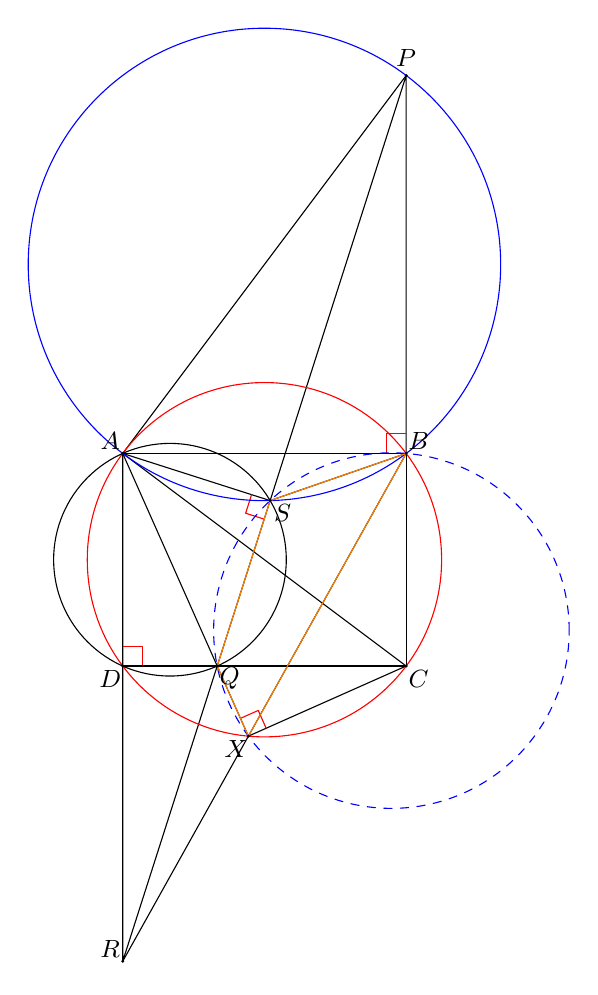
\begin{tikzpicture}[scale=0.45,line cap=round,line join=round]
  \draw[] (-4,3)--(4,-3);
  \draw[] (-4,3)--(4,13.66667);
  \draw[] (-4,3)--(0.16062,1.6686)--(4,3);
  \draw[] (4,3)--(4,13.66667)--(-4,-11.33333)--(-4,3);
  \draw[] (-4,3)--(-0.45361,-4.97938)--(4,-3);
  \draw[red] (-0.67698,-4.47679)--(-0.17439,-4.25341)--(0.04899,-4.75601);
  \draw[red] (-0.36321,1.83623)--(-0.53084,1.3124)--(-0.00701,1.14477);
  \draw[red] (-4,-2.45)--(-3.45,-2.45)--(-3.45,-3);
  \draw[red] (3.45,3)--(3.45,3.55)--(4,3.55);
  \draw[] (4,3)--(-4,-11.33333);
  \draw[] (-4,3)--(4,3)--(4,-3)--(-4,-3)--(-4,3);
  \draw[red] (0,0) circle (5);
  \draw[blue] (0,8.33333) circle (6.66667);
  \draw[] (-2.66667,0) circle (3.28295);
  \draw[dashed,blue] (3.58333,-2) circle (5.01733);
  \draw[orange] (4,3)--(0.16062,1.6686)--(-1.33333,-3)--(-0.45361,-4.97938)--(4,3);
  \fill (-4,3) circle (1.3pt);
  \fill (4,3) circle (1.3pt);
  \fill (4,-3) circle (1.3pt);
  \fill (-4,-3) circle (1.3pt);
  \fill (4,13.66667) circle (1.3pt);
  \fill (-1.33333,-3) circle (1.3pt);
  \fill (-4,-11.33333) circle (1.3pt);
  \fill (-0.45361,-4.97938) circle (1.3pt);
  \fill (0.16062,1.6686) circle (1.3pt);
  \node[font=\small] at (-4.35355,3.35355) {$A$};
  \node[font=\small] at (4.35355,3.35355) {$B$};
  \node[font=\small] at (4.35355,-3.35355) {$C$};
  \node[font=\small] at (-4.35355,-3.35355) {$D$};
  \node[font=\small] at (4,14.16667) {$P$};
  \node[font=\small] at (-0.97978,-3.35355) {$Q$};
  \node[font=\small] at (-4.35355,-10.97978) {$R$};
  \node[font=\small] at (-0.80716,-5.33293) {$X$};
  \node[font=\small] at (0.51417,1.31505) {$S$};
\end{tikzpicture}
\end{center}

Akan dibuktikan bahwa $ABCXD$ siklis. 

Misalkan $X'$ adalah perpotongan $BR$ dengan lingkaran $(ABCD)$. Misalkan pula $Q'$ perpotongan $AX'$ dengan $CD$.

Definisikan $S$ sebagai proyeksi $A$ ke $PQ$. Karena $\angle ASQ = \angle ADQ = 90^\circ$ maka $ASQD$ siklis.

Berarti dengan \textit{power of a point}
$$RX'\cdot RB = RD\cdot DA = RQ\cdot QS.$$
yang menunjukkan bahwa $X'BSQ$ siklis. Berarti $\angle QX'B = \angle PSB$.

Sadari bahwa karena $\angle ABP = \angle PAC$ dan $\angle BCA = \angle PCA$ maka $\triangle BAP \sim \triangle BCA$ yang langsung mengakibatkan $\angle PAB = \angle ACB$.
Sekarang karena $\angle ASP = \angle ABP = 90^\circ$ maka $ASBP$ siklis, sehingga didapat $$\angle PSB = \angle PAB = \angle ACB = \angle AX'B = \angle Q'X'B.$$

Dari kedua fakta tersebut didapat $\angle QX'B = \angle Q'X'B$ yang menunjukkan $Q = Q'$ yang mengakibatkan $X = X'$. Soal terbukti.
\end{proof}
